%
%                       This is a basic LaTeX Template
%                       for the Informatics Research Review

\documentclass[a4paper,11pt]{article}
% Add local fullpage and head macros
\usepackage{head,fullpage}     
% Add graphicx package with pdf flag (must use pdflatex)
\usepackage[pdftex]{graphicx}  
% Better support for URLs
\usepackage{url}
% Date formating
\usepackage{datetime}
% For Gantt chart
\usepackage{pgfgantt}
\usepackage{xcolor}
\usepackage[utf8]{inputenc}


\usepackage{chngpage}

\usepackage{array}


\newdateformat{monthyeardate}{%
  \monthname[\THEMONTH] \THEYEAR}

\parindent=0pt          %  Switch off indent of paragraphs 
\parskip=5pt            %  Put 5pt between each paragraph  
\Urlmuskip=0mu plus 1mu %  Better line breaks for URLs


%                       This section generates a title page
%                       Edit only the following three lines
%                       providing your exam number, 
%                       the general field of study you are considering
%                       for your review, and name of IRR tutor

\newcommand{\examnumber}{B197609}
\newcommand{\field}{Personalized Educational Game in Human-Agent Systems}
\newcommand{\tutor}{Michael Glienecke}
\newcommand{\supervisor}{Nadin Kokciyan}

\begin{document}
\begin{minipage}[b]{110mm}
        {\Huge\bf School of Informatics
        \vspace*{17mm}}
\end{minipage}
\hfill
\begin{minipage}[t]{40mm}               
        \makebox[40mm]{
        
\includegraphics[width=40mm]{crest.png}}
\end{minipage}
\par\noindent
    % Centre Title, and name
\vspace*{2cm}
\begin{center}
        \Large\bf Informatics Project Proposal \\
        \Large\bf \field
\end{center}
\vspace*{1.5cm}
\begin{center}
        \bf \examnumber\\
        \monthyeardate\today
\end{center}
\vspace*{5mm}

%
%                       Insert your abstract HERE
%                       
\begin{abstract}
        The concept of Internet of things(IoT) has been widely known by more and more people in recent years. The potential privacy threats are bright to people due to the characteristic of IoT ecosystem because it may disclose individuals' personal privacy without their awareness. In order to tackle this problem, we plan to design an educational game that could teach people what kind of IoT devices may involve privacy issues and help people better understand their privacy preferences. 
\end{abstract}

\vspace*{1cm}

\vspace*{3cm}
Date: \today

\vfill
{\bf Tutor:} \tutor\\
{\bf Supervisor:} \supervisor
\newpage

%                                               Through page and setup 
%                                               fancy headings
\setcounter{page}{1}                            % Set page number to 1
\footruleheight{1pt}
\headruleheight{1pt}
\lfoot{\small School of Informatics}
\lhead{Informatics Research Review}
\rhead{- \thepage}
\cfoot{}
\rfoot{Date: \date{\today}}
%


\section{Motivation}

In recent years, the concept of Internet of things (IoT), which usually being referred as objects, sensors and everyday items being equipped with network connectivity and 
computing capability \cite{IoT}, has been widely known by more and more people. With the rapid development of human-agent system technologies, people are more gradually engaged with such IoT devices such as voice controller, smartwatch, air quality monitor etc, which are the most popular intelligent agents in these days \cite{IoTdevice}. 

However, the characteristic of IoT ecosystem also determines that it could brings us privacy issues. The IoT ecosystem senses our surrounding like room temperature, reads our biometric data like fingerprint, and transfers those data through smart devices or cloud server. The data collected by IoT devices are usually involved with our personal information, while those data may be shared with others or used for cloud-based big data analysis without our awareness and thus threaten our privacy rights \cite{bigdata}. According to the research conducted by Helen Nissenbaum et al. privacy has been one of the most enduring social issues associated with digital electronic information technologies \cite{privacy}. As such, people need to be more cautious with the privacy policy when deal with IoT data collection.

This project will develop a personalized educational game to users who are usually in touch with IoT devices.The game will be embedded with a privacy preference analyzing model which can provide personalized feedback for users using statistical methods. The proposed development tool for this project is Unity.

\if
Introduce the topic of research and explain its academic and industrial context.

\begin{itemize}
    \item Establish the general subject area.
    \item Describe the broad foundations of your study -- provide adequate background for readers.
    \item Indicate the general scope of your project.
    \item Provide an overview of the sections that will appear in your proposal (optional).
    \item Engage the readers.
\end{itemize}
\fi

\subsection{Problem Statement and Objectives}


Due to the diversity of IoT agents and the complexity of different scenarios in human-agent systems, people have problems correctly identifying the privacy issues caused by IoT devices and being aware of their privacy preference \cite{Alhalafi_2019}, and thus need to face privacy challenges arising from these problems. Some privacy challenges are including user consent acquisition of data collection, and control, customization, and choice of data sharing, as well as the promise of limiting to the stated purpose for the use of collected data \cite{7116422}. In order to fulfill the requirements of tackling this problem, nuanced understanding of societal norms and context, as well as individual preference, are needed \cite{privacy, Beate_2005}.

The main objectives of this project are to develop an educational game that can help people equipped with more knowledge about privacy issue caused by IoT devices and better understand their privacy preferences by analyzing their reactions and attitudes towards privacy choices they were given in different scenarios. Afterwards, an evaluation of these reactions and attitudes will be conducted after people successfully completing the game.




\subsection{Timeliness, Novelty and Significance}

The rapid deployment of IoT technologies has a significant effect on our individual privacy security domain, and hence it is very urgent for everyone to be prepared for the produced corresponding privacy issues, which reflects the timeliness of our project. Even though many kinds of researches so far have explored the factors that affect individual privacy concerns, and made some recommendations on how people should deal with such problems \cite{Lin12expectationand,Tsai09whosviewed,Lederer03whowants,Naeini:2017}, yet there are still few platforms that could educate people and promote them to acquire knowledge of privacy context in a more recreational way, such as educational games. 

In this project, our aim is to use video game to educate people, which proves the novelty of our project. As a study showed that video games engaged study environment can positively impact problem solving skills, promote learning interest, as well as broader knowledge acquisition motivation \cite{unknown}, and nowadays the use of educational games in learning environments becomes increasingly prevalent \cite{Moreno}. Our project will incorporate the current state of study about factors that may impact privacy preference into an entertaining, educational and functional video game. By combining the advantage of game-based learning environment and the timeliness of solving privacy issues in human-agent systems, our project also shows its significance among current works of individual privacy and security.

\if
Explain why the proposed research is of sufficient timeliness and novelty

\subsection{Significance}

The proposal should demonstrate the originality of your intended research. You should therefore explain why your research is important (for example, by explaining how your research builds on and adds to the current state of knowledge in the field or by setting out reasons why it is timely to research your proposed topic) and providing details of any immediate applications, including further research that might be done to build on your findings.
\fi
\subsection{Feasibility}
There are two main parts in the major implementation of this project. One of the parts is to design a game that can perform its educational purpose. It is usually difficult to make a balance between education and entertainment \cite{Moreno}. There has been many examples of how to integrate education in games \cite{KIM2009800,CHENG2012669}. In this project, an interactive design will be implemented in order to attract people's attention and let them gain knowledge without getting bored.

The other part of this project is to give personal feedback of privacy concerns specifically for IoT devices according to people's response when they are facing different situations. We plan to build a privacy preference analyzing model and based on previous study, use algorithm to find the most significant factors that can influence individual privacy concerns and expectations.


\subsection{Beneficiaries}

The beneficiaries of this project could be considered in two points of view. Firstly, for users who have completed this game, they will gain more knowledge about the concept of IoT technologies, as well as the brought potential privacy issues. Secondly, for researchers working in the area of individual privacy and security, our project could provide some insights about people's attitudes and comfort levels in a variety of IoT data collection scenarios.


% Describe how the research will benefit other researchers in the field and in related disciplines. What will be done to ensure that they can benefit? 


\section{Background and Related Work}

In this section, the required background information regarding the project will be introduced with explanations of some important concepts, and some related work will be briefly summarized. Specifically, we will introduce and give some examples of educational games, and factors that may impact privacy preference, as well as the basic knowledge of methods we used for preference analyzing.

\subsection{Educational Games}
In traditional mindset, video games are used for entertainment and recreation, and usually be considered harmful for students. Being addicted to video games could be harmful to both mental and physical health. However, if we appropriately take the advantage of video games, we could achieve more with less in the aspect of education. Bokyeong Kim et al. designed a meta-cognitive strategies in game-based learning to increase student's learning performance \cite{KIM2009800}. What's more, Ching-Hsue Cheng et al. developed a game-based learning system for students and the results shows that students with game-based learning acquired more learning motivations than those with traditional face-to-face teaching \cite{CHENG2012669}.

There are also some public-oriented educational games, among which one of the most famous examples is \textit{Universe Sandbox}. Developed by Giant Army LLC, \textit{Universe Sandbox} is a physics-based space simulator which enables people explore solar system, simulate gravity, and model earth's climate \cite{Universe}. This is a very successful educational game that helps players understand astronomical knowledge and the composition of universe. Another example is \textit{Minecraft: Education Edition}, a well-known sandbox video game developed by Mojang Studios. The education edition of this game is created by TeacherGaming LLC and used for STEM and project-based learning as well as virtual diverse regions exploration \cite{minecraft}.

\subsection{Factors Impacting Privacy Preference}
Outside of the IoT context, there has been many researches focusing on the factors that could be important on determining individual privacy expectations and preference. These studies analyzed the factors based on individual's willingness to share data by measuring the comfort levels associated with sharing data. For example, Lin et al. conducted a research on data collection of privacy-sensitive resource on mobile devices and they concluded that both users' expectations of usage of mobile apps' sensitive resource and the purpose of why sensitive resource are requested by which apps have major impacts on users' privacy decisions \cite{Lin12expectationand}. Furthermore, Tsai et al. did some studies on people's willingness to share data when they are giving feedback, and the results show that people are more comfortable with sharing data when adequate feedback are given \cite{Tsai09whosviewed}.

There are also studies that are more closely related with privacy issues in IoT data collection. Lederer et al. investigated the impacts of the inquirer, namely the device type of collecting data and situations in which data is being collected and they found that privacy preference are more likely to be affected by inquirer than by situation \cite{Lederer03whowants}. In order to better understand people's attitude towards IoT data collection, Naeini et al. conducted a privacy context research by asking people's privacy preference on different scenarios and used machine learning method to built a model to predict their privacy preference \cite{Naeini:2017}.

\subsection{Statistical Correlation Coefficients}

In this project we will build models to analyze individual's privacy preference which are influenced by many factors. Hence statistical methods are required for implementing the models. In the research of Naeini et al. they constructed a generalized linear mixed model (GLMM) with random intercept per participant \cite{Naeini:2017}. The criterion of model selection was based on Bayesian Information Criterion (BIC) which approximates the model's fitness to the data \cite{doi:10.1198/016214504000000269}.

We could also use correlation coefficient to represent the relationships between the significance level of each factor and individual's reaction. There are three famous correlation coefficients in the field of statistics: Pearson product-moment correlation coefficient (PPMCC), Kendall rank correlation coefficient (KRCC), and Spearman's rank correlation coefficient (SRCC). PPMCC, alsno known as simple correlation, measures the distance of the linear relationship between two variables\cite{ref1}. Since the relationship of variables in our project is nonlinear, and PPMCC is usually used for continuous variables, we can't adapt it as the basis of our privacy preference analyzing model. Moreover, KRCC can be applied to discrete variables because it aims to measure the correlation of ordinal variables \cite{Puka2011}, and hence is suitable for calculating individual's comfort level. Additionally, SRCC is used for categorical variables \cite{ref2}, which is also advisable in this project. 

% Demonstrate a knowledge and understanding of past and current work in the subject area, including relevant references like this \cite{template}.


\section{Programme and Methodology}

This section will cover the methodology for implementing the algorithm we used in the preference analyzing model, and how we are going to design the programme for the whole project.

\subsection{Designation of the Game}

The main body of the game will consist of two parts, the interactive part and the privacy question part. The game will be designed in a way that education and entertainment can be best integrated, and the purpose of the interactive part is to make our programme more entertaining and attractive to people. We will use a classical puzzle game, \textit{Spot the difference}, as the backbone of the interactive part. The rules for \textit{Spot the difference} are to find the differences between two similar pictures in a limit time. There are millions versions of \textit{Spot the difference}, and it can be customized by changing the background or any detail of the images. In our project, to be more closely aligned with our educational purpose, we decide to choose images which represent different scenarios in the privacy context. Overall speaking, the scenarios can be categorized according to the location at which privacy issues may happen. The locations are home, public restroom, library, department store and workplace respectively. At the beginning of the puzzle, players can choose which location they want to go and corresponding scenarios will show up.

Both images and text will be used to simulate IoT scenarios. The images, as the main body of \textit{Spot the difference} game, would also provide backgrounds for IoT scenarios. The images will show contextual factors affecting preference, such as locations. Some IoT devices will also be provided in the images but they need to be correctly identified by players. Other contextual factors will be shown in text format by asking privacy questions to players.

We will design three game levels for each of 5 locations mentioned above, and hence there are totally 15 stages. In each game stage, players need to find all differences between two images before the time limitation reaches. The remaining time will convert into points earned, and the goal for players is to achieve points as higher as possible. We also provide the means to get bonus points. If the players successfully spot any IoT agent that may involve privacy issues hidden in pictures, they will gain bonus points. Each picture will hide some certain number of IoT agents waiting for players to discover. We would also provide several tips to help players identify those IoT agents. The game level designation follows the good level design practice proposed by Fares Kayali et al: balancing risk and reward to give players risk incentive \cite{Kayali}. As level increases, the difficulty of spotting the difference as well as identifying the IoT agents will also increase. Correspondingly, more bonus points will be given to the players.

\subsection{Code Book of Factors Impacting Preferences}

In the research of Naeini et al. they analyzed the factors that can impact individual's privacy preference and ranked these factors according to their BIC values \cite{Naeini:2017}. The factors with the lowest BIC value have the most significant level of impacting preference. Based on the significance level, we decide to choose five factors that have the greatest influence:
\begin{itemize}
\item Location: Where the IoT data is collected
\item Device type: What kind of IoT agents is collecting data
\item Retention: How long the collected data will be kept
\item Purpose: How the collected data will be used
\item Being shared: Whether the collected data is being shared with others
\end{itemize}

In the privacy question part of this game, we will present several scenarios in which IoT data is being collected for players and ask them their decisions to allow or deny the collection and their comfort level with data collection. The different data collection scenarios are consist of the combinations of factors impacting preferences. A list of factors and different levels of the factors presented in scenarios, as well as the factor code are showed in table \ref{tab:factors}.

\begin{table}[tb]
\vskip 3mm
\begin{center}
\begin{adjustwidth}{0cm}{0cm}
\begin{tabular}{ |p{.2\textwidth}| p{.8\textwidth}|}
\hline
\textbf{Factors} & \textbf{Levels(code)}\\
\hline
Location    & home(h), public restroom(pr), library(l), department store(cs), workplace(w) \\
\hline
Device type & smartwatch(sw), camera(c), iris scanner(is), smartphone(sp), facial recognition(fr),\ presence sensor(ps), temperature sensor(ts), fingerprint scanner(fs)\\
\hline
retention & unspecified(us), not deleted(nd), purpose satisfied(ps), week(w), year(y)\\
\hline
purpose & A-E different specific purpose will be mentioned\\
\hline
being shared & shared(Y), not shared(N)\\

\hline
\end{tabular}
\end{adjustwidth}
\caption{List of factors, different levels of factors, and their factor code}
\label{tab:factors}
\end{center}
\vskip -3mm
\end{table}

We will use the scenarios dataset of IoT privacy survey conducted by Naeini et al. to simulate different situations \cite{Naeini:2017}. The scenarios are partially contextual depended depending on the game stage where players are currently at. For example, in the interactive part of this game, if a player choose department store as the location, and the hidden IoT agents at this game stage are camera, facial recognition and finger printer scanner, the simulated situation will always happened at department store, and the device type will always be one of the hidden IoT agents, camera, facial recognition or finger printer scanner. In order words, the location and device type are fixed at each stage. The purpose of this design is to induce immersive experiences for players and deepen their memory. 

\subsection{Privacy Preference analyzing Model}

Using the code book, we will encode the factors in one-hot format, a technique to represent categorical variables as binary vectors, which is very commonly used in machine learning \cite{Hancock}. This helps us better deal with the parameters in analyzing privacy preference. We will collect and analyze the responses to privacy questions when the player finishes all stages of the game. The responses could be encoded in binary for allow or deny decision of data collecting, and in ordinal for comfort level, as showed in table \ref{tab:responses}.

\begin{table}[htbp]
    \begin{center}
    \begin{adjustwidth}{0cm}{0cm}
    \begin{tabular}{ |p{.3\textwidth}| p{.7\textwidth}|}
        \hline
        \textbf{Responses} & \textbf{Variable Type}\\
        \hline
        Allow/Deny Decision& Binary: allow(1), deny(0)\\
        \hline
        Comfort Level & Ordinal: Very uncomfortable(0), Uncomfortable(1), Neither comfortable nor uncomfortable(2), Comfortable(3), Very comfortable(4)\\
        \hline
        \end{tabular} 
        \end{adjustwidth}
    \end{center}
    \caption{The variable type of responses to privacy questions}
    \label{tab:responses}
\end{table}

We will use Kendall rank correlation coefficient(KRCC), also known as Kendall's tau, to calculate the correlations between factors and allow/deny decisions as well as the comfort level. There are three formulas to calculate Kendall's tau, in this project we will use tau-b, the most general one to calculate correlations. The equation for tau-b is showed below:
\begin{equation}
    \tau_{b} = \frac{C-D}{\sqrt{T-T_{r}}\sqrt{T-T_{c}}}
\end{equation}

In this equation, C represents the number of concordant pairs where variables change in the same way, and D represents the number of discordant pairs where variables change in the opposite way. Furthermore, $T_{r}$ and $T_{c}$ represent the number of rows and columns respectively \cite{Puka2011}.

% \begin{itemize}
%     \item Detail the methodology to be used in pursuit of the research and justify this choice.
%     \item Describe your contributions and novelty and where you
%     will go beyond the state-of-the-art (new methods, new tools,
%     new data, new insights, new proofs,...)
%     \item Describe the programme of work, indicating the research to be undertaken and the milestones that can be used to measure its progress.
%     \item Where suitable define work packages and define the dependences
%     between these work packages. WPs and their dependences should be
%     shown in the Gantt chart in the research plan.
%     \item Explain how the project will be managed.
%     \item State the limitations of your research.
% \end{itemize}

\subsection{Implementation Details}

Figure \ref{fig:my_label} shows the flowchart of the game. At the home page, players can choose to play the game, or check the scoreboard and their privacy preference feedback. The scoreboard will record the highest score the players reached at each level, and the preference feedback will show when all levels for every location are cleared. Players can repeat each level if they want to achieve higher score. There is an option to skip the privacy question part if the players have completed that question. However, if they want to do the questions again, the preference analyzing results will be covered by new answers.

When players start the game, they will be guided to five locations as they chose. Each location has 3 difficult levels available for players. If they failed to find all different places, they will return to the level selection page, and an \textit{easy mode} will be available for players. In \textit{easy mode}, all different places will be much easier to find, but the score will not be logged. There will be 3 privacy questions after players successfully clear one stage. Afterward, they will be returned to location selection page for the next round of play.


\begin{figure}
    \centering
    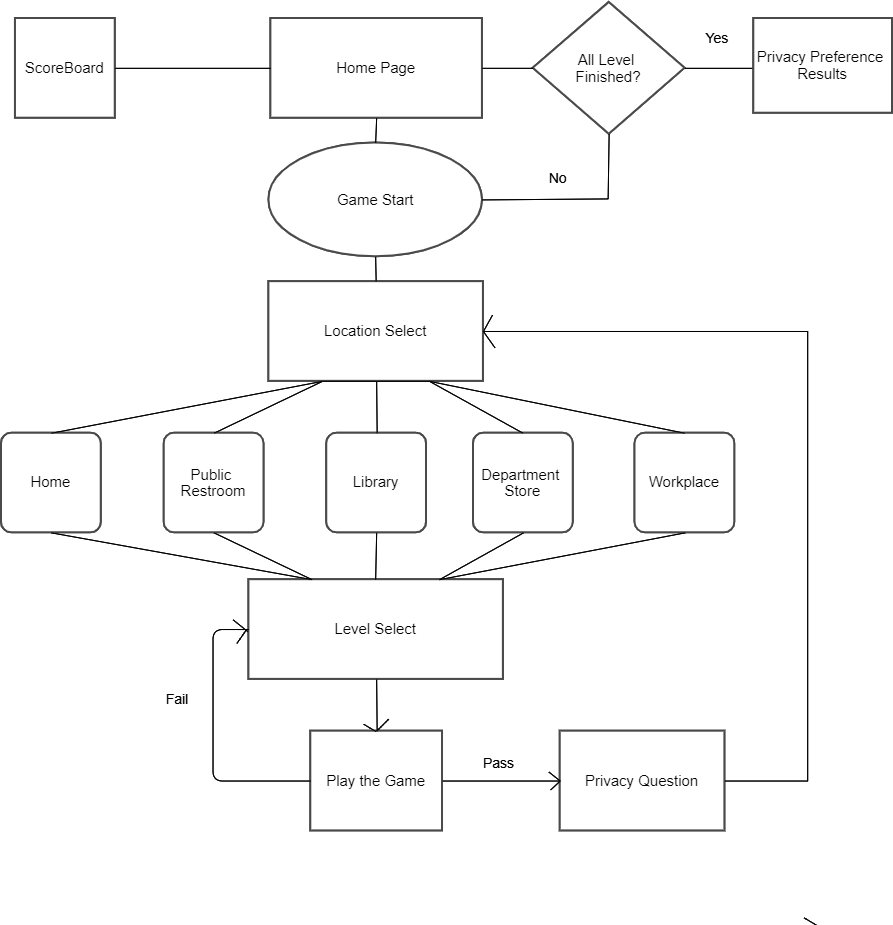
\includegraphics[scale=0.33]{Diagram.png}
    \caption{The flowchart of the game}
    \label{fig:my_label}
\end{figure}


\subsection{Ethics}

Ethical considerations will be taken into account in this project, since we will evaluate the performance of this educational game by collecting user feedback when they complete the game. A Participant Information Sheet (PIS) will be provided for everyone who will play the game. An ethics application will be applied for us to legally conduct the user study. Participants who intend to play this game will need to install this game to their personal computers and consent the PIS before they entering the game.



\section{Evaluation}

We will put a questionnaire link at the end of game to collect their feedback. The questionnaire consists of two parts just like the game. In the first part, we will ask some questions about the gameplay, including the game difficulty, level designations, the context of the game, as well as improvements that should be made etc. In the second part, we will ask some questions about the privacy issues, including whether players gain more knowledge about IoT agents, whether they found themselves becoming more familiar with their privacy preference, whether the individual preference analyzing model helped them make privacy decision in the future, and so on.

% \begin{itemize}
%     \item Describe the specific methods of data collection.
%     \item Explain how you intent to analyze and interpret the results.
% \end{itemize}

% \section{Expected Outcomes}

% The primary expected outcome of this project is that we could provide a good platform that educates people to better understand privacy contexts as well as their privacy preference.

% Conclude your research proposal by addressing your predicted outcomes. What are you hoping to prove/disprove? Indicate how you envisage your research will contribute to debates and discussions in your particular subject area:

% \begin{itemize}
%     \item How will your research make an original contribution to knowledge?
%     \item How might it fill gaps in existing work? 
%     \item How might it extend understanding of particular topics?
% \end{itemize}


\section{Research Plan, Milestones and Deliverables}


Figure \ref{fig:gantt} shows the gantt chart of the activities defined for this project. In the first three weeks, I'm going to do some literature reviews about privacy and IoT domains, as well as study the Unity game engine. I will learn the basic knowledge that can support finishing a whole completed game. In the beginning of the game implementation stage, I will spend a few days on making some graphic materials such as drawing the images for spotting differences. As the most difficult part, it will take me more than 4 weeks to implement the game. On late July, I will start performance evaluation by collecting feedback from participants. The writing of the dissertation will come across all the summer.

\definecolor{barblue}{RGB}{153,204,254}
\definecolor{groupblue}{RGB}{51,102,254}
\definecolor{linkred}{RGB}{165,0,33} 

\begin{figure}[htbp]
\begin{ganttchart}[
    y unit title=0.4cm,
    y unit chart=0.5cm,
    vgrid,hgrid,
    x unit=1.55mm,
    time slot format=isodate,
    title/.append style={draw=none, fill=barblue},
    title label font=\sffamily\bfseries\color{white},
    title label node/.append style={below=-1.6ex},
    title left shift=.05,
    title right shift=-.05,
    title height=1,
    bar/.append style={draw=none, fill=groupblue},
    bar height=.6,
    bar label font=\normalsize\color{black!50},
    group right shift=0,
    group top shift=.6,
    group height=.3,
    group peaks height=.2,
    bar incomplete/.append style={fill=green}
   ]{2018-06-01}{2018-08-16}
   \gantttitlecalendar{month=name}\\
   \ganttbar[
    progress=100,
    bar progress label font=\small\color{barblue},
    bar progress label node/.append style={right=4pt},
    bar label font=\normalsize\color{barblue},
    name=pp
   ]{Background Reading}{2018-06-01}{2018-06-22} \\
\ganttset{progress label text={}, link/.style={black, -to}}
\ganttgroup{Game Implementation}{2018-06-22}{2018-07-20} \\
\ganttbar[progress=4, name=T1A]{Make game materials}{2018-06-22}{2018-06-27} \\
\ganttlinkedbar[progress=0]{Game stage implementation}{2018-06-28}{2018-07-15} \\
\ganttlinkedbar[progress=0]{Privacy question design}{2018-07-16}{2018-07-20} \\
\ganttgroup{Performance Evaluation}{2018-07-21}{2018-08-05} \\
\ganttbar[progress=15, name=T2A]{Collect users feedback}{2018-07-21}{2018-07-28} \\
\ganttlinkedbar[progress=0]{Game evaluation}{2018-07-29}{2018-08-05} \\
\ganttgroup{Dissertation}{2018-07-01}{2018-08-16} \\
  \ganttbar[progress=0]{Writing}{2018-07-01}{2018-08-16}
  \ganttset{link/.style={green}}
  \ganttlink[link mid=.4]{pp}{T1A}
  \ganttlink[link mid=.159]{pp}{T2A}
\end{ganttchart}
\caption{Gantt Chart of the activities defined for this project.}
\label{fig:gantt}
\end{figure}

\begin{table}[htbp]
    \begin{center}
        \begin{tabular}{|c|c|l|}
        \hline
        \textbf{Milestone} & \textbf{Week} & \textbf{Description} \\
        \hline
        $M_1$ & 3 & Game engine knowledge acquired, feasibility confirmed \\
        $M_2$ & 7 & Game implementation completed \\
        $M_3$ & 8 & All participants completed the game, and feedback received  \\
        $M_4$ & 9 & Performance evaluation completed \\
        $M_5$ & 11 & Submission of dissertation \\
        \hline
        \end{tabular} 
    \end{center}
    \caption{Milestones defined in this project.}
    \label{fig:milestones}
\end{table}

\begin{table}[htbp]
    \begin{center}
        \begin{tabular}{|c|c|l|}
        \hline
        \textbf{Deliverable} & \textbf{Week} & \textbf{Description} \\
        \hline
        $D_1$ & 7 & Game first version released \dots\\
        $D_2$ & 9 & Performance evaluation completed  \dots\\
        $D_3$ & 11 & Dissertation \\
        \hline
        \end{tabular} 
    \end{center}
    \caption{List of deliverables defined in this project.}
    \label{fig:deliverables}
\end{table}


%                Now build the reference list
\bibliographystyle{unsrt}   % The reference style
%                This is plain and unsorted, so in the order
%                they appear in the document.

{\small
\bibliography{main}       % bib file(s).
}
\end{document}

% \if
% \begin{itemize}
%     \item Answer the question:''What is the gap that needs to be filled?"
%     and/or ''What is the problem that needs to be solved?"
%     \item State the problem clearly early in a paragraph.
%     \item Limit the variables you address in stating your problem.
%     \item Consider bordering the problem as a question.
% \end{itemize}


% \subsection{Research Hypothesis and Objectives}

% Identify the overall aims of the project and the individual measurable objectives against which you would wish the outcome of the work to be assessed. Clearly spell out any research hypothesis you are following.

% Include a justification (rationale) for the study. Be clear about what your study will not address.
% \fi
